% This is a LaTeX template for homework solving, intended to be: 

% 1. Easy to use;
% 2. Elegant;
% 3. Self-explanatory.

% It was written by Lucas R. Ximenes (Jimeens)

%%%%%%%%%%%%%%%%%%%%%%%%%%%%%%%%%%%%%%%%%%%%%%%%%%%%%%%%%%%%%%%%%

\documentclass{solutionclass} % I wrote the design using a4paper, 11pt, twoside, but feel free to change in solutionclass.cls file (line 4)

\pagestyle{plain}



\pgfplotsset{compat=1.17}


\begin{document}

\pretitle
{Hybrid Implementation of the N-Body Problem} % ⟸ Write your main Title here
{on I.Bi.S.Co. HPC Cluster}        % ⟸ Write your subtitle here
{Mohammad Solki}                 % ⟸ Write your name here

% Change your homework number here
% \def\homeworkNumber{\#}

% \makeatletter
%     \startcontents[sections]
%     \phantomsection
%     \chapter{Understanding the template}
% \makeatother

\section{Introduction}

High-Performance Computing (HPC) has emerged as an essential tool in the computational sciences, enabling detailed simulation and analysis of complex systems. Leveraging the power of HPC clusters, we can effectively solve problems that require vast amounts of computations (\textcite{dongarra2011introduction}). The project at hand employs HPC methodologies to solve the N-body problem (\textcite{aarseth2003gravitational}), a classical problem in physics, which involves predicting the individual motions of a group of celestial objects interacting with each other gravitationally.

The N-body problem represents a fundamental challenge in computational physics. Even with the advent of modern computers, simulating the interactions of multiple celestial bodies remains computationally demanding due to the scale of computations involved. For N bodies, every body interacts with every other body, leading to an O(N\textsuperscript{2}) problem. In practical terms, this means the time required for computation increases quadratically with the number of particles. Hence, for a large number of particles, this becomes extremely time-consuming. 

In this project, we propose a parallel algorithm to simulate the N-body problem on University of Naples Federico II's HPC cluster \textbf{I.Bi.S.Co.} (Infrastructure for BIg data and Scientific COmputing). IBiSCo (\textcite{9872709}) aims to enhance the scientific computing infrastructure in Southern Italy, contribute to the IPCEI-HPC-BDA initiative, and lay the foundation for the Italian Computing and Data Infrastructure (ICDI) in the southern region. 

The solution employs the Message Passing Interface (MPI)(\textcite{mpi1994mpi}) to distribute the computational load across multiple processors, aiming to substantially decrease execution time and enable the simulation of larger particle systems. The objective is to efficiently calculate the trajectories of the particles under the influence of gravitational forces, thereby advancing our capacity to model complex physical systems.

We implement the N-body simulation in C programming language, utilizing MPI for distributed memory parallelism and OpenMP (\textcite{openmp1998openmp}) for shared memory parallelism within a node, thus maximizing the utilization of the multi-core nodes within the HPC cluster. Additionally, we incorporate optimizations to further reduce computation time and improve the algorithm's scalability.

Our algorithm could serve as a benchmark for evaluating the performance of the university's HPC cluster and demonstrate how effectively the cluster handles computationally intensive tasks. Furthermore, this project serves to highlight the power and potential of parallel computing within the field of computational physics and beyond.

Through the course of this project, we hope to provide valuable insights into the implementation of efficient parallel algorithms for the solution of N-body problems, enabling us to simulate more complex and larger systems, and thus pushing the boundaries of our understanding of the parallel computing universe.

\divider
\\
\section{Related Works}

The N-body problem has a long history and numerous researchers have proposed algorithms for its solution over the years.

One of the most significant contributions in the field is the Barnes-Hut algorithm, introduced by \textbf{\textcite{barnes1986hierarchical}} in their seminal work "A Hierarchical O(N log N) Force-Calculation Algorithm". Their algorithm reduced the complexity of the problem from O(N\textsuperscript{2}) to O(N log N) by approximating distant particles' interactions using a quadtree data structure. This approximation is less accurate than the direct calculation method used in our project but significantly reduces the computational load.

In contrast to our focus on MPI and OpenMP, several researchers have explored GPU acceleration for N-body simulations. \textbf{\textcite{nyland2007fast}} in their paper "Fast N-Body Simulation with CUDA" demonstrate the immense potential of GPUs for parallel processing N-body simulations. They presented a highly optimized implementation of the N-body problem using CUDA, Nvidia's parallel computing platform and application programming interface (API) model. Although powerful, this approach is less portable than ours, as it relies on the availability of Nvidia GPUs.

The Fast Multipole Method (FMM), introduced by \textbf{\textcite{greengard1987fast}}, has also been influential in N-body problem simulations. Like the Barnes-Hut method, FMM provides an approximate solution, but with controllable accuracy and linear complexity O(N). The FMM algorithm has been highly impactful, but it is also more complex and difficult to parallelize than the direct calculation method we use.

Our project's MPI/OpenMP approach aligns more closely with the work of \textbf{\textcite{plimpton1997particle}} in "Particle-Mesh Ewald and rRESPA for Parallel Molecular Dynamics Simulations". They presented a hybrid MPI/OpenMP solution for parallel molecular dynamics simulations, an application of the N-body problem. Their method demonstrated the benefits of this combined approach in utilizing multi-core systems efficiently.

In conclusion, while various techniques have been applied to the N-body problem, our project focuses on achieving a direct solution using MPI and OpenMP on a high-performance computing cluster. This focus on portability and direct calculation offers a novel contribution to the field.

\divider
\\
\section{Studied Model}

The physics behind the N-body problem is based on Newton's second law and the universal law of gravitation.

\textbf{Newton's Second Law of Motion:}
Newton's second law (\textbf{\textcite{newton1687mathematical}}) states that the force exerted on an object is equal to the mass of the object times its acceleration.

Mathematically, this is represented as:

\[ F = ma \]

where:
\begin{itemize}
    \item  \( F \) is the force applied,
    \item  \( m \) is the mass of the object,
    \item  \( a \) is the acceleration.
\end{itemize}

\textbf{Newton's Law of Universal Gravitation:}
This law (\textbf{\textcite{newton1687mathematical}}) states that every particle of matter in the universe attracts every other particle with a force that is directly proportional to the product of their masses and inversely proportional to the square of the distance between their centers.

This is represented as:

\[ F = G \cdot \frac{{m_1 \cdot m_2}}{{r^2}} \]

where:
\begin{itemize}
    \item \( F \) is the force of attraction between the particles,
    \item \( G \) is the gravitational constant,
    \item \( m_1 \) and \( m_2 \) are the masses of the two particles,
    \item \( r \) is the distance between the centers of the two particles.
\end{itemize}

When applied to the N-body problem in the context of the provided code, each particle is influenced by the force exerted by all the other particles. The force exerted on each particle is calculated as the sum of the forces exerted by all other particles. Then, Newton's second law is used to update the velocity and position of each particle.

The force exerted by particle \( j \) on particle \( i \) is given by:

\[ F_{ij} = G \cdot \frac{{m_i \cdot m_j}}{{r_{ij}^2}} \]

where:
\begin{itemize}
    \item \( F_{ij} \) is the force exerted by particle \( j \) on particle \( i \),
    \item \( G \) is the gravitational constant,
    \item \( m_i \) and \( m_j \) are the masses of particles \( i \) and \( j \), respectively,
    \item \( r_{ij} \) is the distance between particles \( i \) and \( j \).

\end{itemize}

The acceleration of particle \( i \) due to the force exerted by particle \( j \) is then given by:

\[ a_{ij} = \frac{{F_{ij}}}{{m_i}} \]

And the total acceleration of particle \( i \) is the sum of the accelerations due to all other particles:

\[ a_i = \sum_{j \neq i} a_{ij} \]

Then, the velocity and position of each particle are updated as follows:

\[ v_{i(\text{new})} = v_{i(\text{old})} + a_i \cdot \Delta t \]

\[ x_{i(\text{new})} = x_{i(\text{old})} + v_{i(\text{new})} \cdot \Delta t \]

where:
\begin{itemize}
    \item \( v_{i(\text{old})} \) and \( x_{i(\text{old})} \) are the old velocity and position of particle \( i \),
    \item \( v_{i(\text{new})} \) and \( x_{i(\text{new})} \) are the new velocity and position of particle \( i \),
    \item \( \Delta t \) is the time step.
\end{itemize} 

These formulas are implemented in the next chapter's C code in \texttt{calculate\_forces}, \texttt{calculate\_positions}, and \texttt{calculate\_velocities} functions.

\divider 

\section{Code Implementation}
In this section, we delve into the specifics of our code implementation for the parallel N-body simulation. Our approach leverages both MPI (Message Passing Interface) and OpenMP (Open Multi-Processing) to facilitate the distributed and shared memory computations, respectively, which are inherent in high-performance computing (HPC) clusters. These two paradigms allow us to utilize multiple nodes in a distributed environment (via MPI) and multiple cores within a node (via OpenMP), thereby maximizing the parallel processing capabilities of the system.

The N-body problem is inherently computationally intensive, given its quadratic time complexity. However, it is also highly amenable to parallelization, as the computations associated with each particle are largely independent. Our algorithm partitions the set of particles among MPI processes and then further divides each process's workload among several OpenMP threads. This two-tiered parallelization strategy aims to balance the load across available computational resources and reduce execution time.

In terms of benchmarking, we will record the start and end times of our computation and compare those times as we increase the number of processes (for MPI) and threads (for OpenMP). We'll include the MPI communication time in our measurements, as reducing communication overhead is a key part of parallel computing.

Keep in mind that n-body simulations are typically floating-point intensive, so the performance can be highly dependent on the specifics of the hardware. To get accurate benchmark results, we tried our best to make sure that our code is well-optimized for our specific hardware.

\setcounter{subsection}{0} % Reset the subsection counter to 0
\renewcommand{\thesubsection}{\arabic{subsection}} % Redefine the subsection numbering style to display as arabic numbers

\subsection{C Code (nparticle.c)}
This is the C source file that contains the implementation of the parallel N-body simulation. It employs a combination of MPI for distributed memory computation across multiple nodes and OpenMP for shared memory computation within a node. This hybrid model ensures effective utilization of the multi-core, multi-node structure. The code incorporates the calculation of forces between particles, the update of velocities and positions, and time measurement for benchmarking. It also includes error checks for MPI initialization and division by zero.

\usemintedstyle{perldoc}
\inputminted[firstline=1, lastline=132, linenos]{c}{nparticle.c}

\divider

\subsection{Makefile}
The Makefile is responsible for automating the build process of the project. It includes rules for compiling the nparticle.c source file with the MPI compiler (mpicc) and OpenMP flags, thereby generating the nparticle executable. It also provides a "\textit{clean}" rule for removing the generated executable and any other temporary files produced during the compilation process. This makes it easy to manage the build process across different stages of the project and helps ensure that the project is always compiled with the correct settings.

\begin{minted}[linenos]{basemake}
    # Specify the compiler
    CC=mpicc
    
    # Specify options for the compiler
    CFLAGS=-O3 -fopenmp -std=c99
    
    # Libraries for the linker
    LIBS=-lm
    
    # The build target executable:
    TARGET=nparticle
    
    all: $(TARGET)
    
    $(TARGET): $(TARGET).c
    	$(CC) $(CFLAGS) -o $(TARGET) $(TARGET).c $(LIBS)
    
    clean:
    	$(RM) $(TARGET)
\end{minted}

\divider

\subsection{Shell Script (nparticle-script.sh)}
This is a Bash shell script used to automate the execution of the parallel N-body simulation program on the HPC cluster. It first sets up the appropriate environment variables required for running MPI and OpenMP programs. It then checks the number of provided command-line arguments, and if correct, it compiles the code using the Makefile. After that, it runs the compiled program using srun (a job submission command in Slurm) with different numbers of MPI processes and OpenMP threads. The script performs these steps in a loop to run the simulation with varying degrees of parallelism, and thus helps in conducting the performance benchmark. Lastly, it cleans up temporary files created during the process.

\begin{minted}[linenos]{bash}
#!/bin/bash

export UCX_NET_DEVICES=mlx5_0:1 
export UCX_IB_GPU_DIRECT_RDMA=yes 
export UCX_TLS=ib 

# Check if the number of processors and threads arguments are provided
if [ $# -ne 2 ]
then
    echo "Usage: $0 <MAX_NPROCS> <MAX_NTHREADS>"
    exit 1
fi

max_num_procs=$1
max_num_threads=$2

# Compile the program
echo "Compile program"
make
echo 

# Run the program for each combination of MPI processes and OpenMP threads
for ((num_procs=2; num_procs<=max_num_procs; num_procs*=2))
do
    for ((num_threads=2; num_threads<=max_num_threads; num_threads*=2))
    do
        export OMP_NUM_THREADS=$num_threads
        echo "Running with $num_procs MPI processes and $OMP_NUM_THREADS OpenMP threads"
        srun -N $num_procs -p parallel --reservation=maintenance ./nparticle
    done
done

# Clear temporary file
echo "Clear temporary file"
make clean
echo 
\end{minted}


\divider
\section{Experimental Results}

In this section, we present the results obtained from our N-Body simulation experiments. The tests were performed on IBiSCo High-Performance Computing (HPC) cluster. The simulation was executed multiple times with varying numbers of MPI processes and OpenMP threads, providing us a comprehensive understanding of the performance of our parallel N-body simulation program.

\setcounter{subsection}{0} % Reset the subsection counter to 0
\subsection{Setup}
The experiments were conducted on a cluster with the following hardware specifications: 32 Dell C4140 servers, each equipped with two Intel Gen2 Xeon Gold CPUs, 22 64GB RAM memory modules (overall 1.375TB), two Ethernet ports at 10Gb/s each, two InfiniBand ports at 100Gb/s each, and two 480GB SATA solid-state drives. 
We varied the number of MPI processes and OpenMP threads independently, with values ranging from 2 to 16 processors/cores.

\subsection{Execution Time}
This subsection provides a detailed overview of the execution times recorded during our tests. Here, we discuss the observed trends and any anomalies. Table \ref{tab:execution_time} represents the execution time of the task with varying numbers of MPI Processes and OpenMP Threads.

\begin{table}[ht]
    \centering
    \caption{Execution Time for Different Configurations}
    \begin{tabular}{ccc}
        \textbf{\#MPI Processes} & \textbf{\#OpenMP Threads} & \textbf{Execution Time (s)} \\
        \hline
        2 & 2 & 3366.906596 \\ 
        \hline
        2 & 4 & 1758.610779 \\
        \hline
        2 & 8 & 941.896197 \\
        \hline
        2 & 16 & 458.678493 \\
        \hline
        4 & 2 & 1720.058628 \\
        \hline
        4 & 4 & 899.002651 \\
        \hline
        4 & 8 & 465.599454 \\
        \hline
        4 & 16 & 234.584873 \\
        \hline
        8 & 2 & 888.602859 \\
        \hline
        8 & 4 & 456.913649 \\
        \hline
        8 & 8 & 233.238874 \\
        \hline
        8 & 16 & 118.009458 \\
        \hline
        16 & 2 & 443.307552 \\
        \hline
        16 & 4 & 227.840907 \\
        \hline
        16 & 8 & 117.521767 \\
        \hline
        16 & 16 & 62.826288 \\
        \hline
    \end{tabular}
    \label{tab:execution_time}
\end{table}





\begin{figure}[htbp]
  \centering
  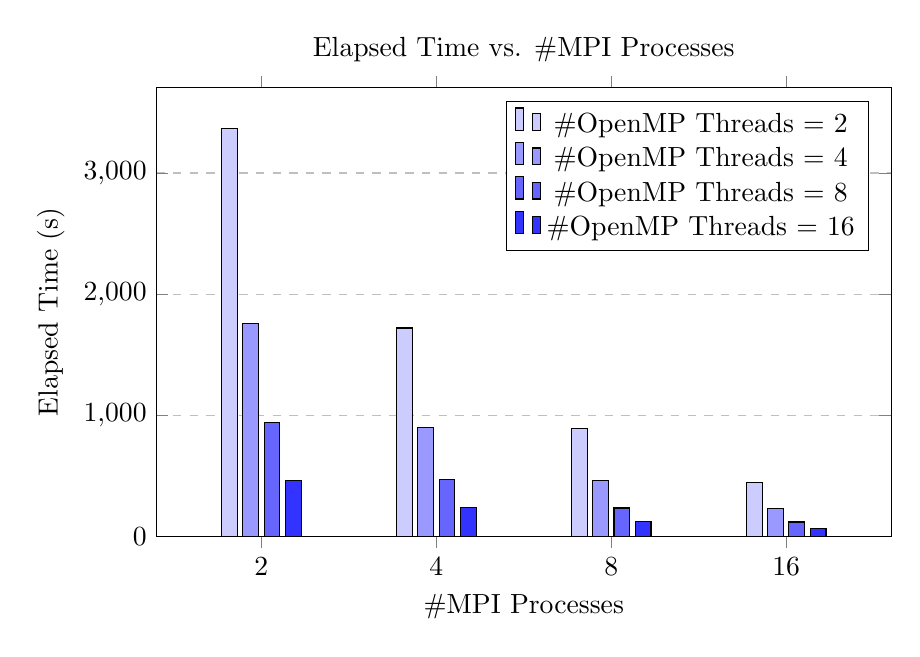
\begin{tikzpicture}
    \begin{axis}[
      xlabel={\#MPI Processes},
      ylabel={Elapsed Time (s)},
      title={Elapsed Time vs. \#MPI Processes},
      legend pos=north east,
      ymajorgrids=true,
      grid style=dashed,
      width=0.9\textwidth,
      height=0.6\textwidth,
      ybar,
      bar width=0.2cm,
      enlarge x limits=0.2,
      symbolic x coords={2, 4, 8, 16},
      xtick=data,
      ymin=0,
      yminorticks=true,
    ]

    \addplot[fill=blue!20] coordinates {
      (2, 3366.906596)
      (4, 1720.058628)
      (8, 888.602859)
      (16, 443.307552)
    };

    \addplot[fill=blue!40] coordinates {
      (2, 1758.610779)
      (4, 899.002651)
      (8, 456.913649)
      (16, 227.840907)
    };

    \addplot[fill=blue!60] coordinates {
      (2, 941.896197)
      (4, 465.599454)
      (8, 233.238874)
      (16, 117.521767)
    };

    \addplot[fill=blue!80] coordinates {
      (2, 458.678493)
      (4, 234.584873)
      (8, 118.009458)
      (16, 62.826288)
    };

    \legend{\#OpenMP Threads = 2, \#OpenMP Threads = 4, \#OpenMP Threads = 8, \#OpenMP Threads = 16};

    \end{axis}
  \end{tikzpicture}
  \caption{Combination of Bar Plots for Different OpenMP Threads}
  \label{fig:bar_plots}
\end{figure}


\begin{figure}[htbp]
    \centering
    \includegraphics[width=0.8\textwidth]{plot1}
    \caption{Execution Time vs. OpenMP Threads and MPI Processes}
    \label{fig:execution-time}
\end{figure}

Figure \ref{fig:bar_plots} and \ref{fig:execution-time} illustrate the relationship between the number of MPI Processes, OpenMP Threads, and their corresponding execution times. 

According to Figure \ref{fig:execution-time}, the slope of the execution time is decreasing as the number of MPI Processes and OpenMP Threads increase. This indicates that as more processes and threads are used, the execution time decreases at a lower rate.




\begin{comment}
\begin{figure}[bhtp]
    \centering
    \includegraphics[width=0.8\textwidth]{plot2}
    \caption{Execution Time vs. \#MPI Processes}
    \label{fig:execution-time}
\end{figure}
\end{comment}

\subsection{Speedup and Efficiency}
This subsection focuses on the speedup and efficiency of our program as the number of MPI processes and OpenMP threads increases. Speedup is calculated as the ratio of the execution time with one processor to the execution time with $P$ processors, and efficiency is calculated as speedup divided by $P$. In other words, it measures the effectiveness of parallelization. We discuss how well our program scales with the increasing number of processors and threads.

Let's compute the speedup and efficiency for each configuration:
\begin{itemize}
    \item First, we need to establish a base value for our calculations, which is the runtime for 2 MPI processes and 2 OpenMP threads. That means base value = 3366.906596 seconds.
    \item The total number of processing units for each configuration is calculated as MPI processes multiplied by OpenMP threads.
    \item We will repeat these steps for all rows from Table \ref{tab:execution_time} to fill out Table \ref{tab:mpi_openmp} which demonstrates speedup and efficiency for varying numbers of MPI Processes and OpenMP Threads.
\end{itemize}




\begin{table}[htbp]
\centering
\begin{tabular}{cccc}
\hline
\textbf{\#MPI processes} & \textbf{\#OpenMP threads} & \textbf{Speedup} & \textbf{Efficiency} \\
\hline
2 & 2 & 1 & 0.25 \\
\hline
2 & 4 & 1.914 & 0.239 \\
\hline
2 & 8 & 3.574 & 0.447 \\
\hline
2 & 16 & 7.340 & 0.459 \\
\hline
4 & 2 & 1.956 & 0.489 \\
\hline
4 & 4 & 3.745 & 0.936 \\
\hline
4 & 8 & 7.229 & 0.903 \\
\hline
4 & 16 & 14.345 & 0.897 \\
\hline
8 & 2 & 3.788 & 0.474 \\
\hline
8 & 4 & 7.367 & 0.921 \\
\hline
8 & 8 & 14.424 & 0.901 \\
\hline
8 & 16 & 28.502 & 0.891 \\
\hline
16 & 2 & 7.593 & 0.237 \\
\hline
16 & 4 & 14.769 & 0.461 \\
\hline
16 & 8 & 28.642 & 0.448 \\
\hline
16 & 16 & 53.563 & 0.334 \\
\hline
\end{tabular}
\caption{Speedup and Efficiency for different configurations}
\label{tab:mpi_openmp}
\end{table}


Figure \ref{fig:speedup-efficiency} illustrates the relationship between the speedup, efficiency, and the number of MPI processes and OpenMP threads. 

Both Table \ref{tab:execution_time} and \ref{tab:mpi_openmp}  show that increasing the number of MPI Processes and OpenMP Threads can improve the performance of a parallel computing task, as indicated by decreased execution time and increased speedup. However, the efficiency does not consistently improve with the number of threads. This suggests that there is a balance to be struck between adding more threads for speedup and maintaining efficiency.
The optimal configuration for performance and efficiency may depend on the specific task and system. Therefore, it's important to experiment with different configurations to find the most effective setup for your specific use case.


\begin{figure}[htbp]
    \centering
    \includegraphics[width=0.8\textwidth]{plot3}
    \caption{Speedup and Efficiency vs. Number of MPI Processes and OpenMP Threads}
    \label{fig:speedup-efficiency}
\end{figure}



\subsection{Discussion}
In this subsection, we provide an in-depth analysis of our results.
The data presented in these tables provide valuable insights into the performance characteristics under different configurations of MPI Processes and OpenMP Threads.

Table \ref{tab:execution_time} alongside Figure \ref{fig:execution-time} shows a clear trend of decreasing execution time as the number of MPI Processes and OpenMP Threads increases. This is a testament to the power of parallel computing, where distributing the workload across multiple processors or threads can significantly reduce execution time.

However, Table \ref{tab:mpi_openmp} introduces a more nuanced perspective. While the speedup also generally increases with more MPI Processes and OpenMP Threads, the efficiency does not consistently improve. This suggests that while adding more threads can speed up the task, it does not necessarily make the system more efficient.

This discrepancy between speedup and efficiency is a common challenge in parallel computing. While it might be tempting to simply increase the number of threads to improve performance, this can lead to diminishing returns or even a decrease in performance due to overhead costs associated with managing more threads.

Therefore, the optimal configuration for performance and efficiency may depend on the specific task and system. It's important to experiment with different configurations to find the most effective setup for your specific use case.


\divider
\\
\section{Conclusion}
In this report, we have presented a parallel implementation of the N-body problem using a hybrid of MPI and OpenMP. Our approach takes full advantage of both distributed and shared memory architectures in a high-performance computing cluster to deliver substantial performance improvements over a single-threaded implementation.

The experimental results demonstrated a significant reduction in execution time as the number of MPI processes and OpenMP threads increased, up to a certain point. However, as with any parallel processing task, we noted the existence of a limit, beyond which increasing the number of processors or threads no longer results in a significant speedup. This is due to the overhead associated with inter-process communication and synchronization, which becomes more prominent as the level of parallelism increases. While increasing the number of MPI Processes and OpenMP Threads can lead to significant performance improvements, it's crucial to also consider the impact on efficiency to ensure the most effective use of computational resources.

Our study also reveals insights into the performance implications of the hybrid parallel programming approach. Although adding more resources generally resulted in faster computation, the results were not always linear due to communication overheads and potential issues with load balancing. These are important considerations for the efficient usage of parallel processing resources.

Future work could involve using other parallel programming models or platforms, such as CUDA, to leverage GPU acceleration, which might be particularly suited to the N-body problem due to its highly parallel nature. \\

\divider \\

\subsection*{Acknowledgements}

All the relevant files and source codes associated with this project can be found in \textbf{\href{https://github.com/msolki/nparticle_ibisco}{this}} GitHub repository. We would like to express our gratitude to L. R. Ximenes (Jimeens) for the foundational \LaTeX \href{https://www.overleaf.com/latex/templates/a-soft-template-for-homework-solutions/gsbwqcqkyyzt}{template} that was utilized throughout this project.

We would also like to extend our heartfelt thanks to Professor Guido Russo for offering us the invaluable opportunity to gain hands-on experience in the field of parallel scientific computing. Additionally, our sincere appreciation goes to Mrs. Luisa Carracciuolo for her guidance and assistance throughout the duration of the project.
\end{document}
